%
% $Id: $
%
%
% Compilar a .pdf con LaTeX (pdflatex)
% Es necesario instalar Beamer (paquete latex-beamer en Debian)
%

%
% Gr�ficos:
% Los gr�ficos pueden suministrarse en PNG, JPG, TIF, PDF, MPS
% Los EPS deben convertirse a PDF (usar epstopdf)
%

\documentclass{beamer}
\usetheme{Warsaw}
%\usebackgroundtemplate{
\includegraphics[width=\paperwidth]{format/libresoft-bg.png}}
%\usepackage[spanish]{babel}
\usepackage[latin1]{inputenc}
\usepackage{graphics}
\usepackage{amssymb} % Simbolos matematicos
\usepackage{url}

%\definecolor{libresoftgreen}{RGB}{162,190,43}
%\definecolor{libresoftblue}{RGB}{0,98,143}

%\setbeamercolor{titlelike}{bg=libresoftgreen}

%% Metadatos del PDF.
\hypersetup{
  pdftitle={Automatic Detection of Bad Programming Habits in Scratch: A Preliminary Study},
  pdfauthor={Jes�s Moreno Le�n, Gregorio Robles},
  pdfcreator={GSyC/LibreSoft \\ Universidad Rey Juan Carlos},
  pdfproducer=PDFLaTeX,
  pdfsubject={Learning to code with Scratch. Automatic assesment.},
}
%%

\begin{document}

\title{Automatic Detection of Bad Programming Habits in Scratch}
\subtitle{A Preliminary Study}
\institute{jesus.moreno@programamos.es, grex@gsyc.urjc.es \\
GSyC/Libresoft, Universidad Rey Juan Carlos}
\author{Jes�s Moreno Le�n, Gregorio Robles}
\date{FIE 2014, Madrid, October 23 2014}

\frame{
\maketitle
\begin{center}

\includegraphics[width=2cm]{format/libresoft-logo}
\hspace{0.5cm}

\includegraphics[width=5cm]{format/gsyc-urjc}
\vspace{0.5cm}

\includegraphics[width=3cm]{format/emadrid.png}
\end{center}
}


% Si el titulo o el autor se quieren acortar para los pies de p�gina
% se pueden redefinir aqu�:
%\title{Titulo corto}
%\author{Autores abreviado}

%% LICENCIA DE REDISTRIBUCION DE LAS TRANSPAS
\frame{
~
\vspace{3cm}

\begin{flushright}

\includegraphics[width=2.2cm]{figs/by-sa}

{\tiny
(cc) 2014 Gregorio Robles and Jes�s Moreno Le�n\\
  Some rights reserved. This work licensed under Creative Commons \\
  Attribution-ShareAlike License. To view a copy of full license, see \\
  http://creativecommons.org/licenses/by-sa/3.0/ or write to \\
  Creative Commons, 559 Nathan Abbott Way, Stanford, \\
  California 94305, USA. \\
\ \\
Some of the figures have been taken from the Internet \\
Source, and author and licence if known, is specified. \\
For those images, \emph{fair use} applies.
}
\end{flushright}
}
%%

\section{FIE 2014 - eMadrid Session}


%--------------------------------------------------------
\usebackgroundtemplate{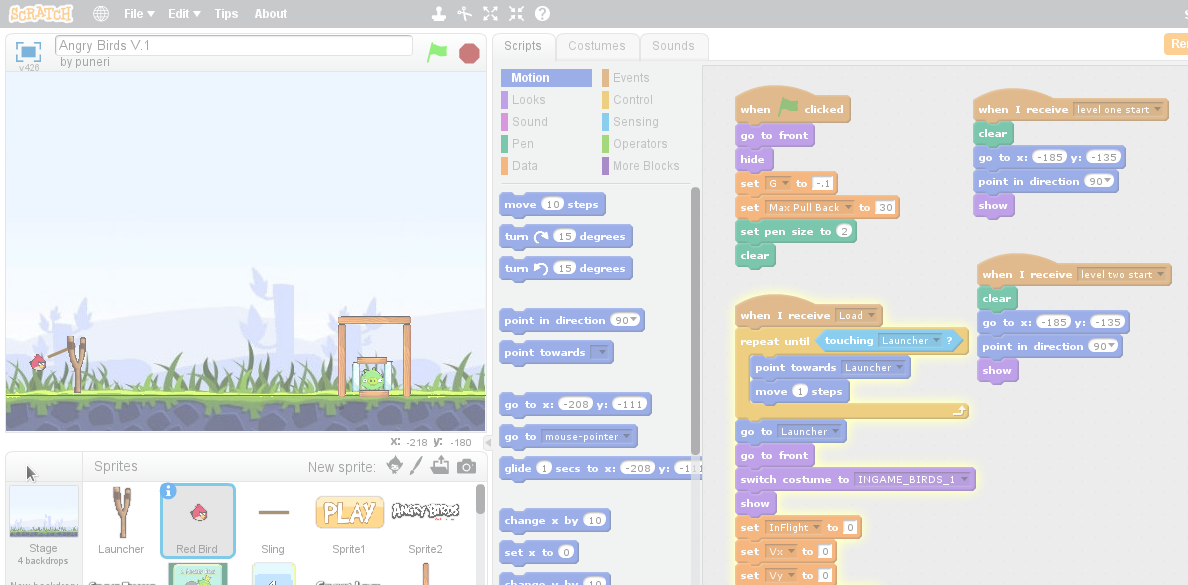
\includegraphics[width=19cm]{figs/AngryBirds.png}}

\begin{frame}
\frametitle{Goal of our paper}

\begin{center}
\Huge {\bf Are bad programming habits a common practice in the Scratch community?}
\end{center}

\end{frame}


%-----------------------    ---------------------------------
\usebackgroundtemplate{
\includegraphics[width=14cm]{figs/audience.png}}
% http://cdn.netrafic.com/wp-content/uploads/2011/02/audience.gif

\begin{frame}
\frametitle{Audience}

Who should/could be interested in this talk?

\begin{itemize}
  \item Educators teaching how to code
  \item Students learning to program
  \item Developers of programming learning tools
\end{itemize} 

\end{frame}

\usebackgroundtemplate{}
%--------------------------------------------------------
\begin{frame}
\frametitle{Scratch}


  \begin{columns}[T]
    \begin{column}{1\textwidth}
     \begin{block}{Learning to code with Scratch}
\begin{itemize}
  \item Scratch has shown to be successfull in teaching basic and advanced programming concepts
  \item However, bad programming habits have been detected
  \item There are no automatic tools to check for \textit{correctness}
  \item \texttt{Hairball}: \texttt{lint}-inspired static analysis of Scratch projects
\end{itemize}
    \end{block}
    \end{column}
    
  \end{columns}

\end{frame}

\usebackgroundtemplate{}

%--------------------------------------------------------
\begin{frame}
\frametitle{Bad programming habits with Scratch (I)}

\begin{figure}[t!]
\begin{center}
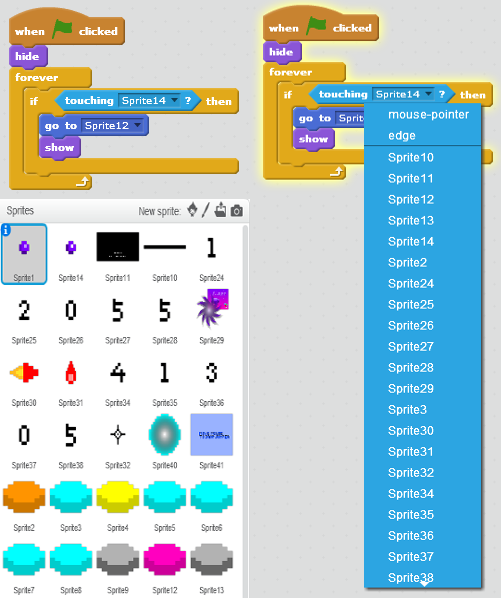
\includegraphics[width=7cm, height=6cm]{figs/SpriteNaming.png}
\end{center}
\label{fig:naming}
\end{figure}

\begin{center}
\emph{Bad}/default naming of sprites
\end{center}
\end{frame}

%--------------------------------------------------------
\begin{frame}
\frametitle{Bad programming habits in Scratch (and II)}

  \begin{columns}[T]
    \begin{column}{0.5\textwidth}
 
     \begin{block}{Example of repeated code}
\begin{figure}[t!]
\begin{center}
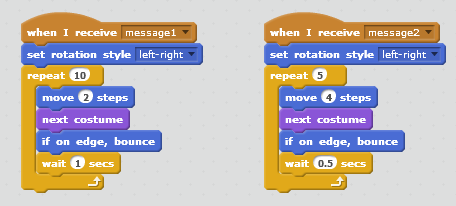
\includegraphics[width=5.4cm,height=2.5cm]{figs/CodeRepetition1.png}
\end{center}
\label{fig:repetition1}
\end{figure}
     \end{block}
    \end{column}
    \begin{column}{0.5\textwidth}
     \begin{block}{Solution to avoid repeated code}
\begin{figure}[t!]
\begin{center}
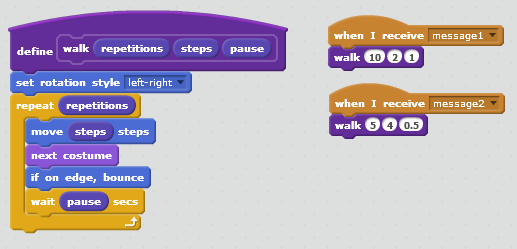
\includegraphics[width=5.4cm,height=2.5cm]{figs/CodeRepetition2.png}
\end{center}
Blocks should be created to avoid repetition of code
\label{fig:repetition2}
\end{figure}
     \end{block}

    \end{column}
  \end{columns}

\end{frame}

%--------------------------------------------------------
%--------------------------------------------------------
\usebackgroundtemplate{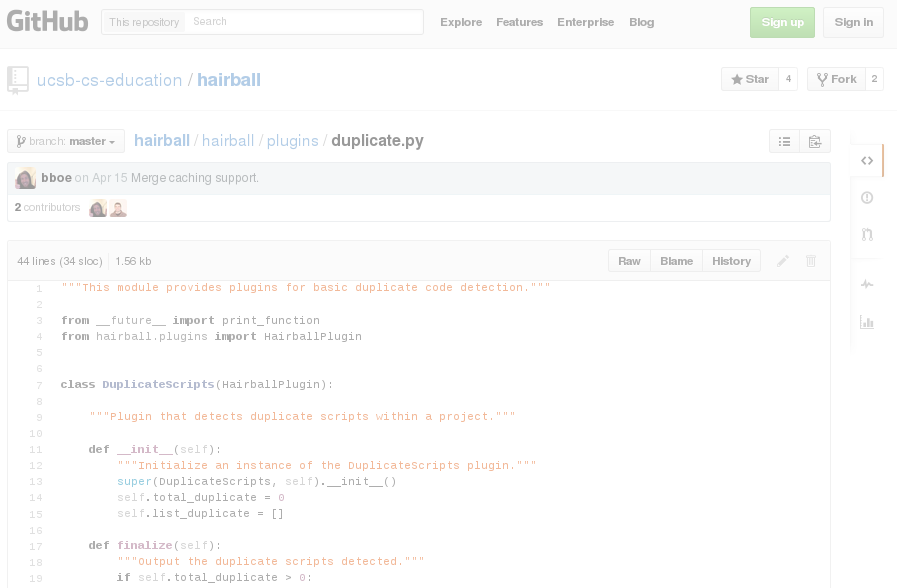
\includegraphics[width=13cm,height=9.2cm]{figs/plugins.png}}
% background: http://25.media.tumblr.com/b83aa72682992ab34b8ce7e61c0cb7f9/tumblr_menxc7qcq61ryin08o1_r1_1280.jpg
\begin{frame}
\frametitle{Hairball plug-ins development}

  \begin{columns}[T]
    \begin{column}{0.8\textwidth}
     \begin{block}{\vspace{0.1cm}\center{We have developed two plug-ins for Hairball to automatically detect bad programming habits}\vspace{0.1cm}}
\vspace{0.3cm}
\begin{enumerate}
  \item convention.SpriteNaming
\vspace{0.15cm}
  \item duplicate.DuplicateScripts
\end{enumerate}
\vspace{0.4cm}
    \end{block}
    \end{column}
  \end{columns}

\end{frame}

\usebackgroundtemplate{}

%--------------------------------------------------------
%\usebackgroundtemplate{\includegraphics[width=13cm]{figs/iceberg.jpg}}
% background: http://www.wim-network.org/wp-content/uploads/2012/04/iceberg.jpg

\begin{frame}
\frametitle{Scratch projects repository analysis}

\begin{table}
\begin{center}
  \begin{tabular}{ | l | c | c | c |}
   \hline
              & Default names & Duplicated scripts & Defined blocks \\ \hline\hline
    Projects & 79 & 62 & 17 \\ \hline
    Mean & 5.94 & 7.23 & 1.11 \\ \hline
 22   Median & 3 & 2 & 0 \\ \hline
    Maximum & 67 & 71 & 25 \\
    \hline    
  \end{tabular}
\end{center}
\caption{Analysis of 100 ramdonly downloaded Scratch projects}
\label{table:results}
\end{table}
\end{frame}

%--------------------------------------------------------
%\usebackgroundtemplate{\includegraphics[width=13cm]{figs/take-away.jpg}}
% background: http://2.bp.blogspot.com/-78Eh4TBpdtU/UPw7ULV73PI/AAAAAAAAHAE/6DQfvPNCo-Y/s1600/8723052-stylized-red-stamp-showing-the-term-take-away-all-on-white-background.jpg
\usebackgroundtemplate{
\includegraphics[width=13cm]{figs/future.png}}

\begin{frame}
\frametitle{Future Work}

\begin{enumerate}
  \item Extend the scope of the study developing new plug-ins
  \item Analyze dataset with 5 years of data from the Scratch website
  \item Dr. Scratch (alpha version): http://drscratch.programamos.es
\end{enumerate}
\vspace{\baselineskip}
\vspace{\baselineskip}
\hfill{\Tiny Background picture: Simon Cunningham }

\end{frame}

%--------------------------------------------------------
%\begin{frame}
%\frametitle{GSyC/LibreSoft}

%\begin{figure}[t!]
%\begin{center}
%\includegraphics[width=11cm]{figs/libresoft.jpg}
%\end{center}
%\label{fig:libresoft}
%\end{figure}

%\begin{center}
%The GSyC/LibreSoft research team at URJC (Madrid).
%\end{center}

%\end{frame}

%--------------------------------------------------------
%\begin{frame}
%\frametitle{Our work at GSyC/LibreSoft}

%\begin{figure}[t!]
%\begin{center}
%\includegraphics[width=2.5cm]{figs/research}
% http://www.memphis.edu/crow/images/research_2.jpg
%\hspace{0.1cm}
%\includegraphics[width=2.5cm]{figs/teaching}
% http://2.bp.blogspot.com/_uxgwfriLwSo/TOWDr8IjaLI/AAAAAAAABLM/d7H-G5jIq-c/s1600/teaching.gif
%\hspace{0.1cm}
%\includegraphics[width=2.5cm]{figs/development}
% http://www.vidadigitalradio.com/wp-content/uploads/2009/04/hackers_cartoons.jpg
%\hspace{0.1cm}
%\includegraphics[width=2.5cm]{figs/promotion}
% http://bloggeate.com/wp-content/uploads/2011/04/como-promocionar-tu-blog.jpg
%\end{center}
%\label{fig:whatwedo}
%\end{figure}

%\begin{center}
%GSyC/LibreSoft's tasks: research, teaching, development, promotion of free software.

%\end{center}
%\end{frame}

\usebackgroundtemplate{}

%--------------------------------------------------------
\frame{
\maketitle
\begin{center}

\includegraphics[width=2cm]{format/libresoft-logo}
\hspace{0.5cm}

\includegraphics[width=5cm]{format/gsyc-urjc}
\vspace{0.5cm}

\includegraphics[width=3cm]{format/emadrid.png}
\end{center}
}

\end{document}
